\section{Projective Geometry}

\subsection{Projective plane}

\begin{frame}[t]
    \frametitle{Projective plane}
     % \begin{minipage}[t]{0.48\linewidth}
     %       \begin{block}{}
     %        The projective plane is a quotient-set define over a vector space without its
     %            origin, and define by an equivalence relation which let
     %    two vector be the same if there are on the same line.
     %       \end{block}
     %    \begin{block}{}
     %        More precisely the projective plane is the reunion between the affine plan and the infinite
     %    line. 
     %    \end{block}
     %    \begin{block}{}
     %        The affine plane is generated by the projective line. We can see an example of a
     %        projective line on the figure \ref{fig:droiteProjective}.
     %    \end{block}
     % \end{minipage}%
    % \hfill%
    % \begin{minipage}[t]{0.48\linewidth}
        \begin{figure}[t]
            \centering
            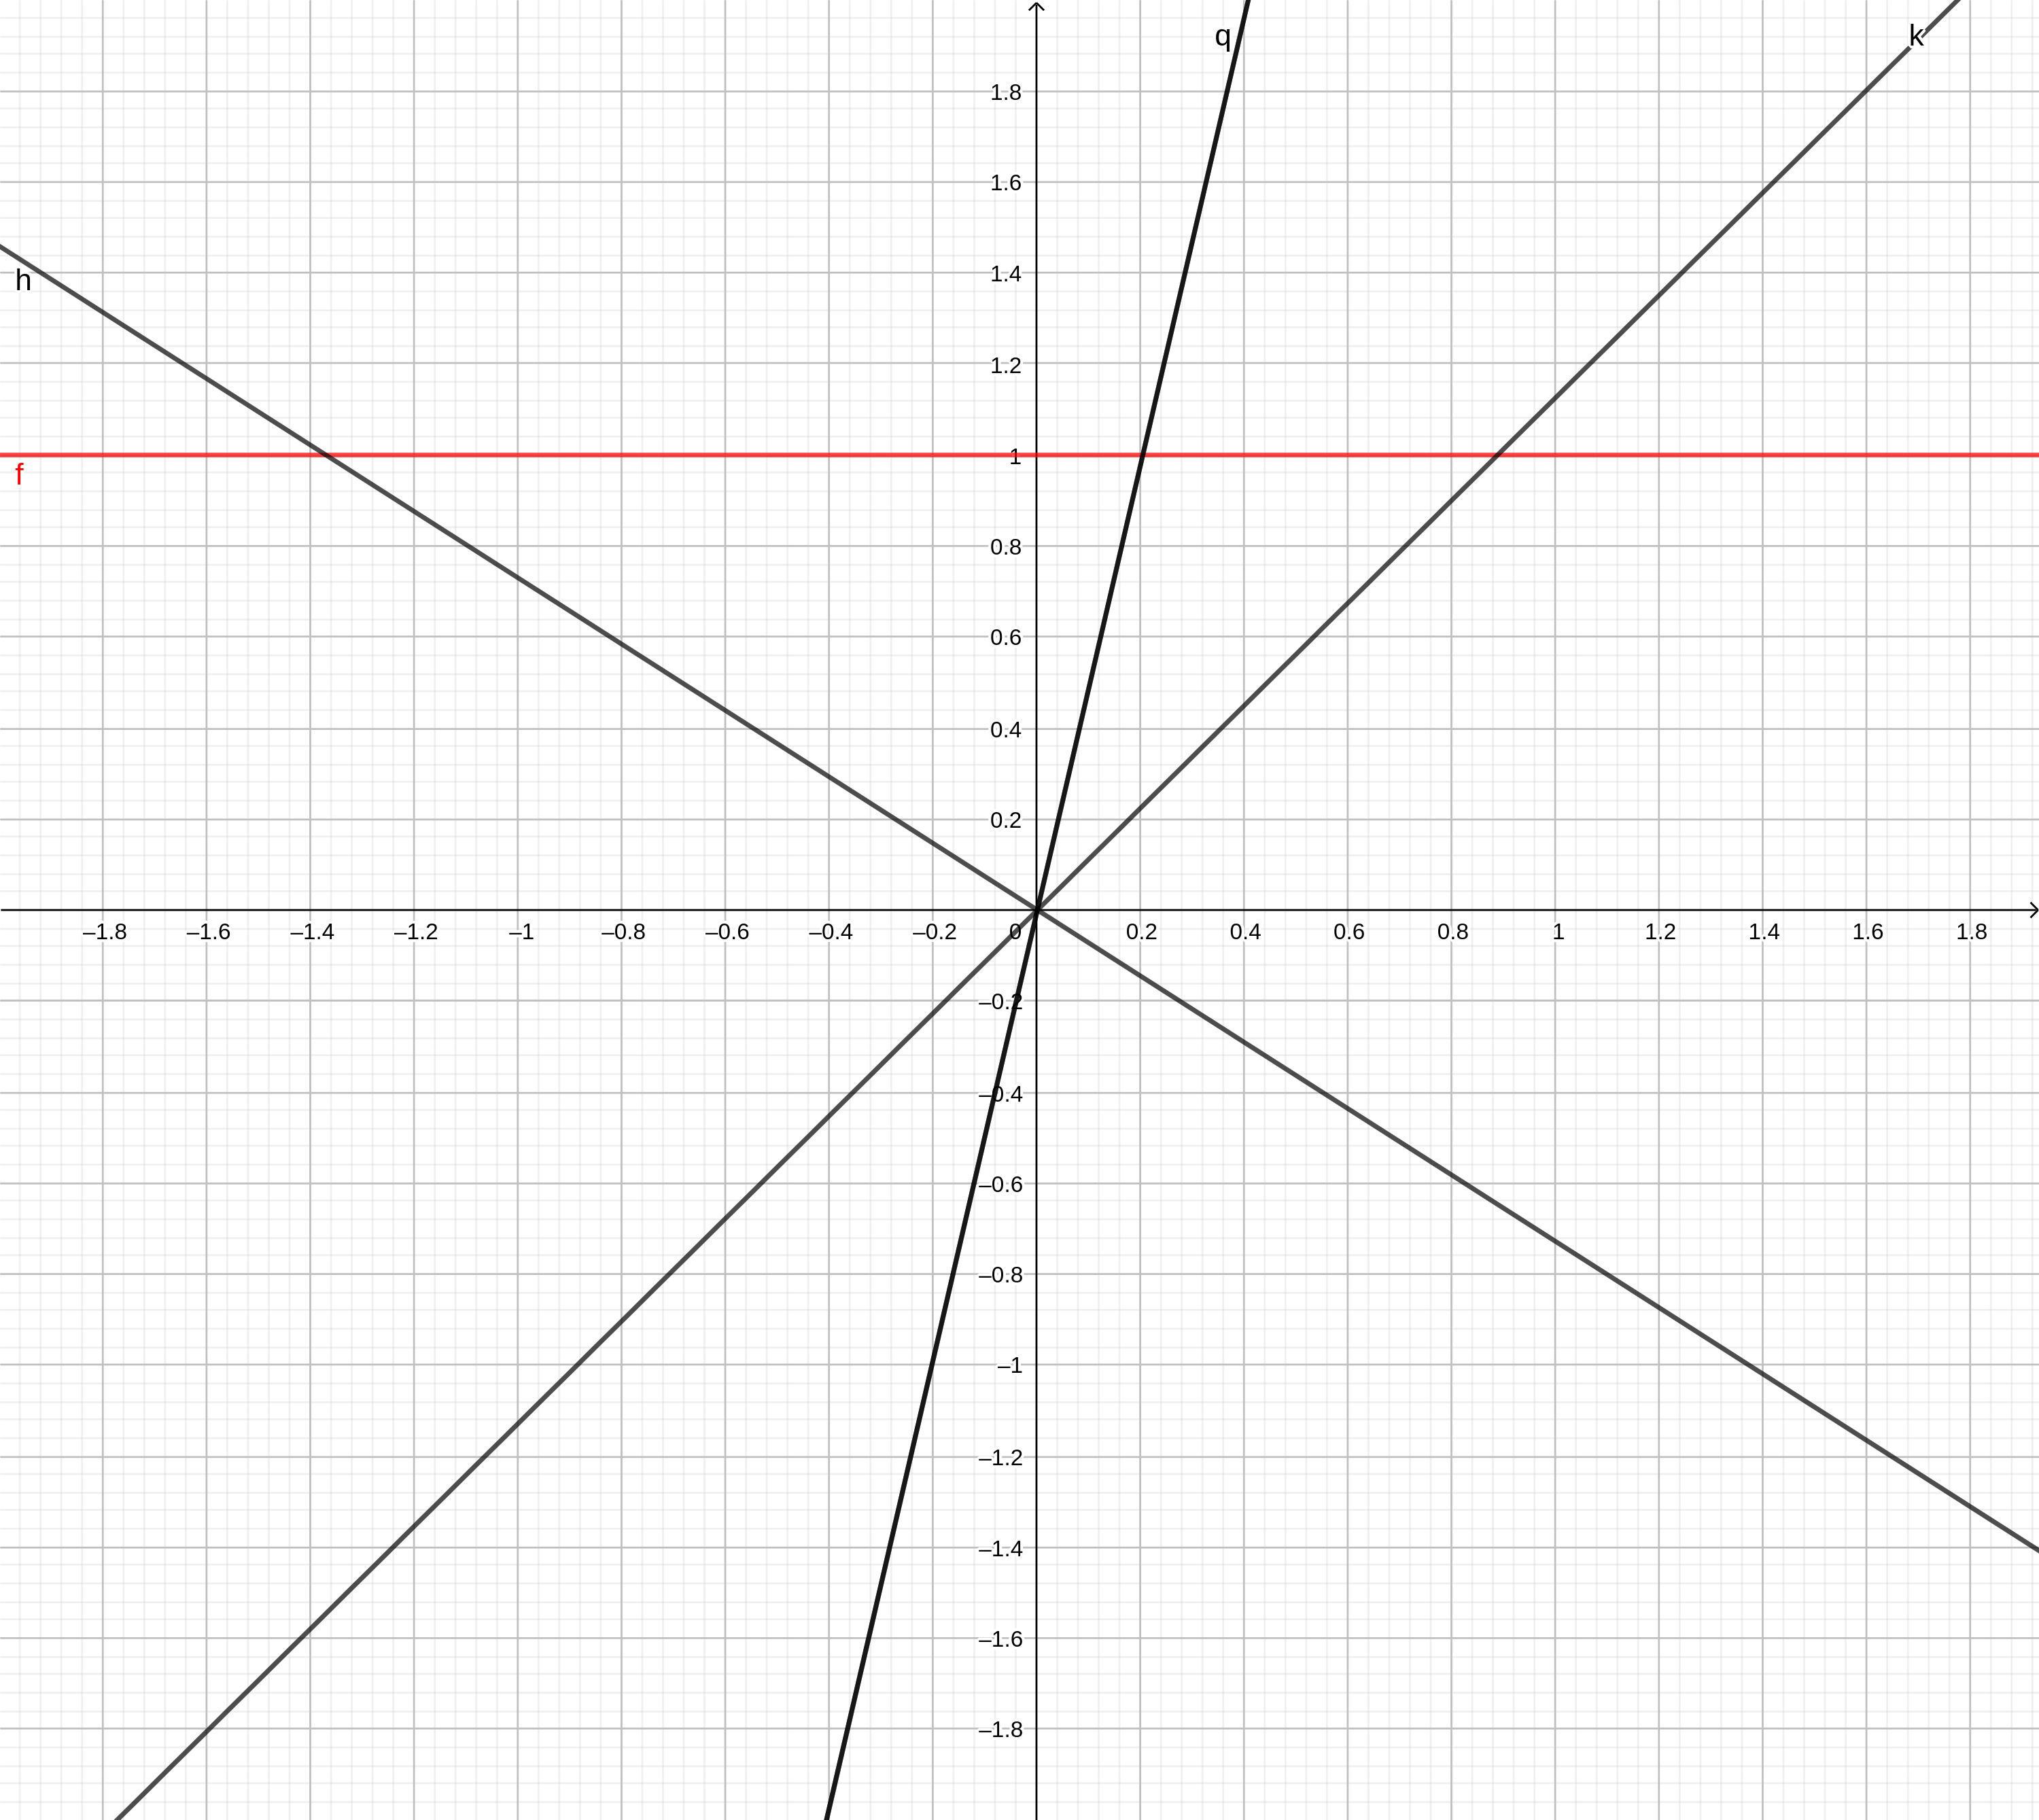
\includegraphics[width=0.4\textwidth]{droiteProjective}
            \caption{Projective line in red}
            \label{fig:droiteProjective}
        \end{figure}
    % \end{minipage}
\end{frame}

\subsection{Affine slice}
\begin{frame}[t]
\frametitle{Affine slice}
% \begin{center}
% Over $\R^3$ we can see the projective line as the line that generates the affine plane.
% As we can see in the following figure \ref{fig:affineSlice}
% \end{center}
\begin{figure}[h]
    \centering
    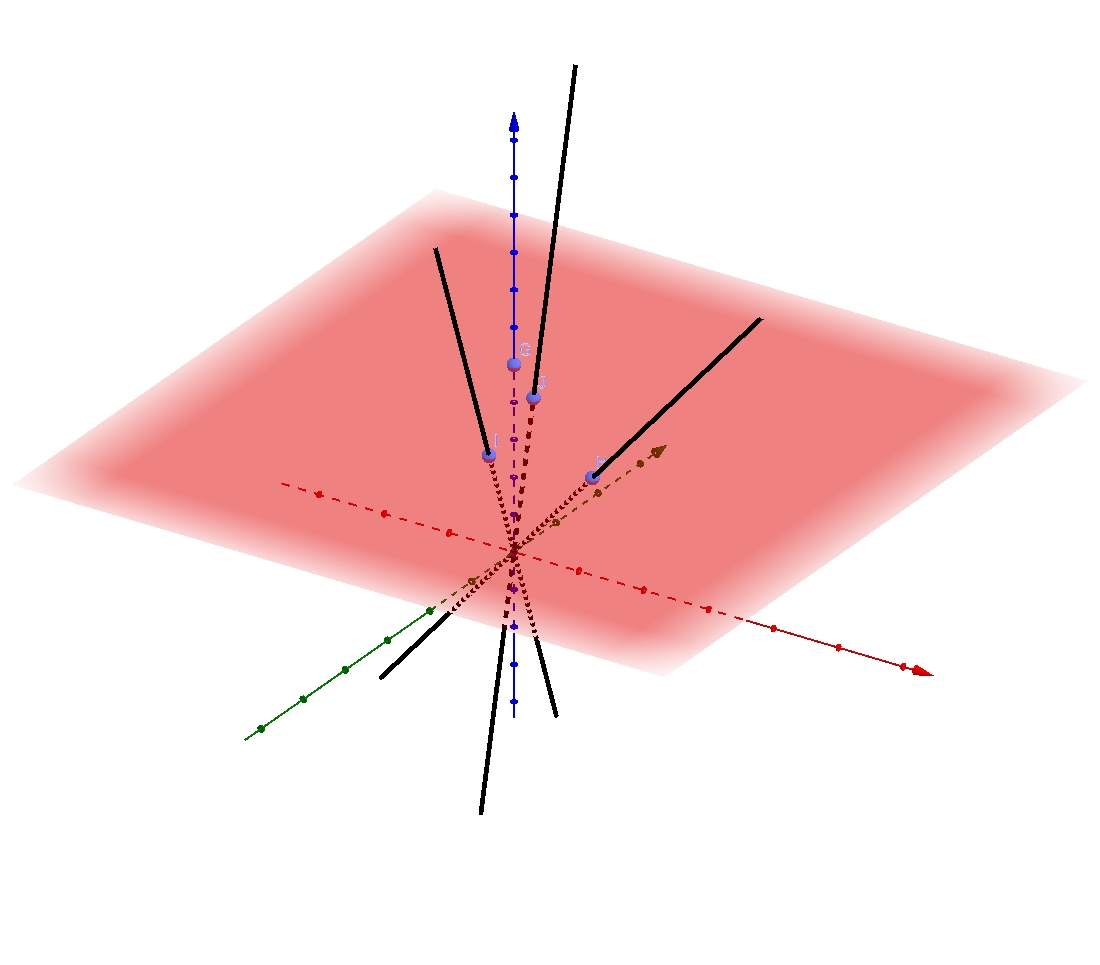
\includegraphics[width=0.5\textwidth]{affineSlice}
    \caption{Affine slice of the projective plane in red}
    \label{fig:affineSlice}
\end{figure}
\end{frame}

\subsection{Projective plane and infinity point}
\begin{frame}[t]
    \frametitle{Affine slice of the projective plan and the infinity point}
        \begin{figure}[h]
            \centering
            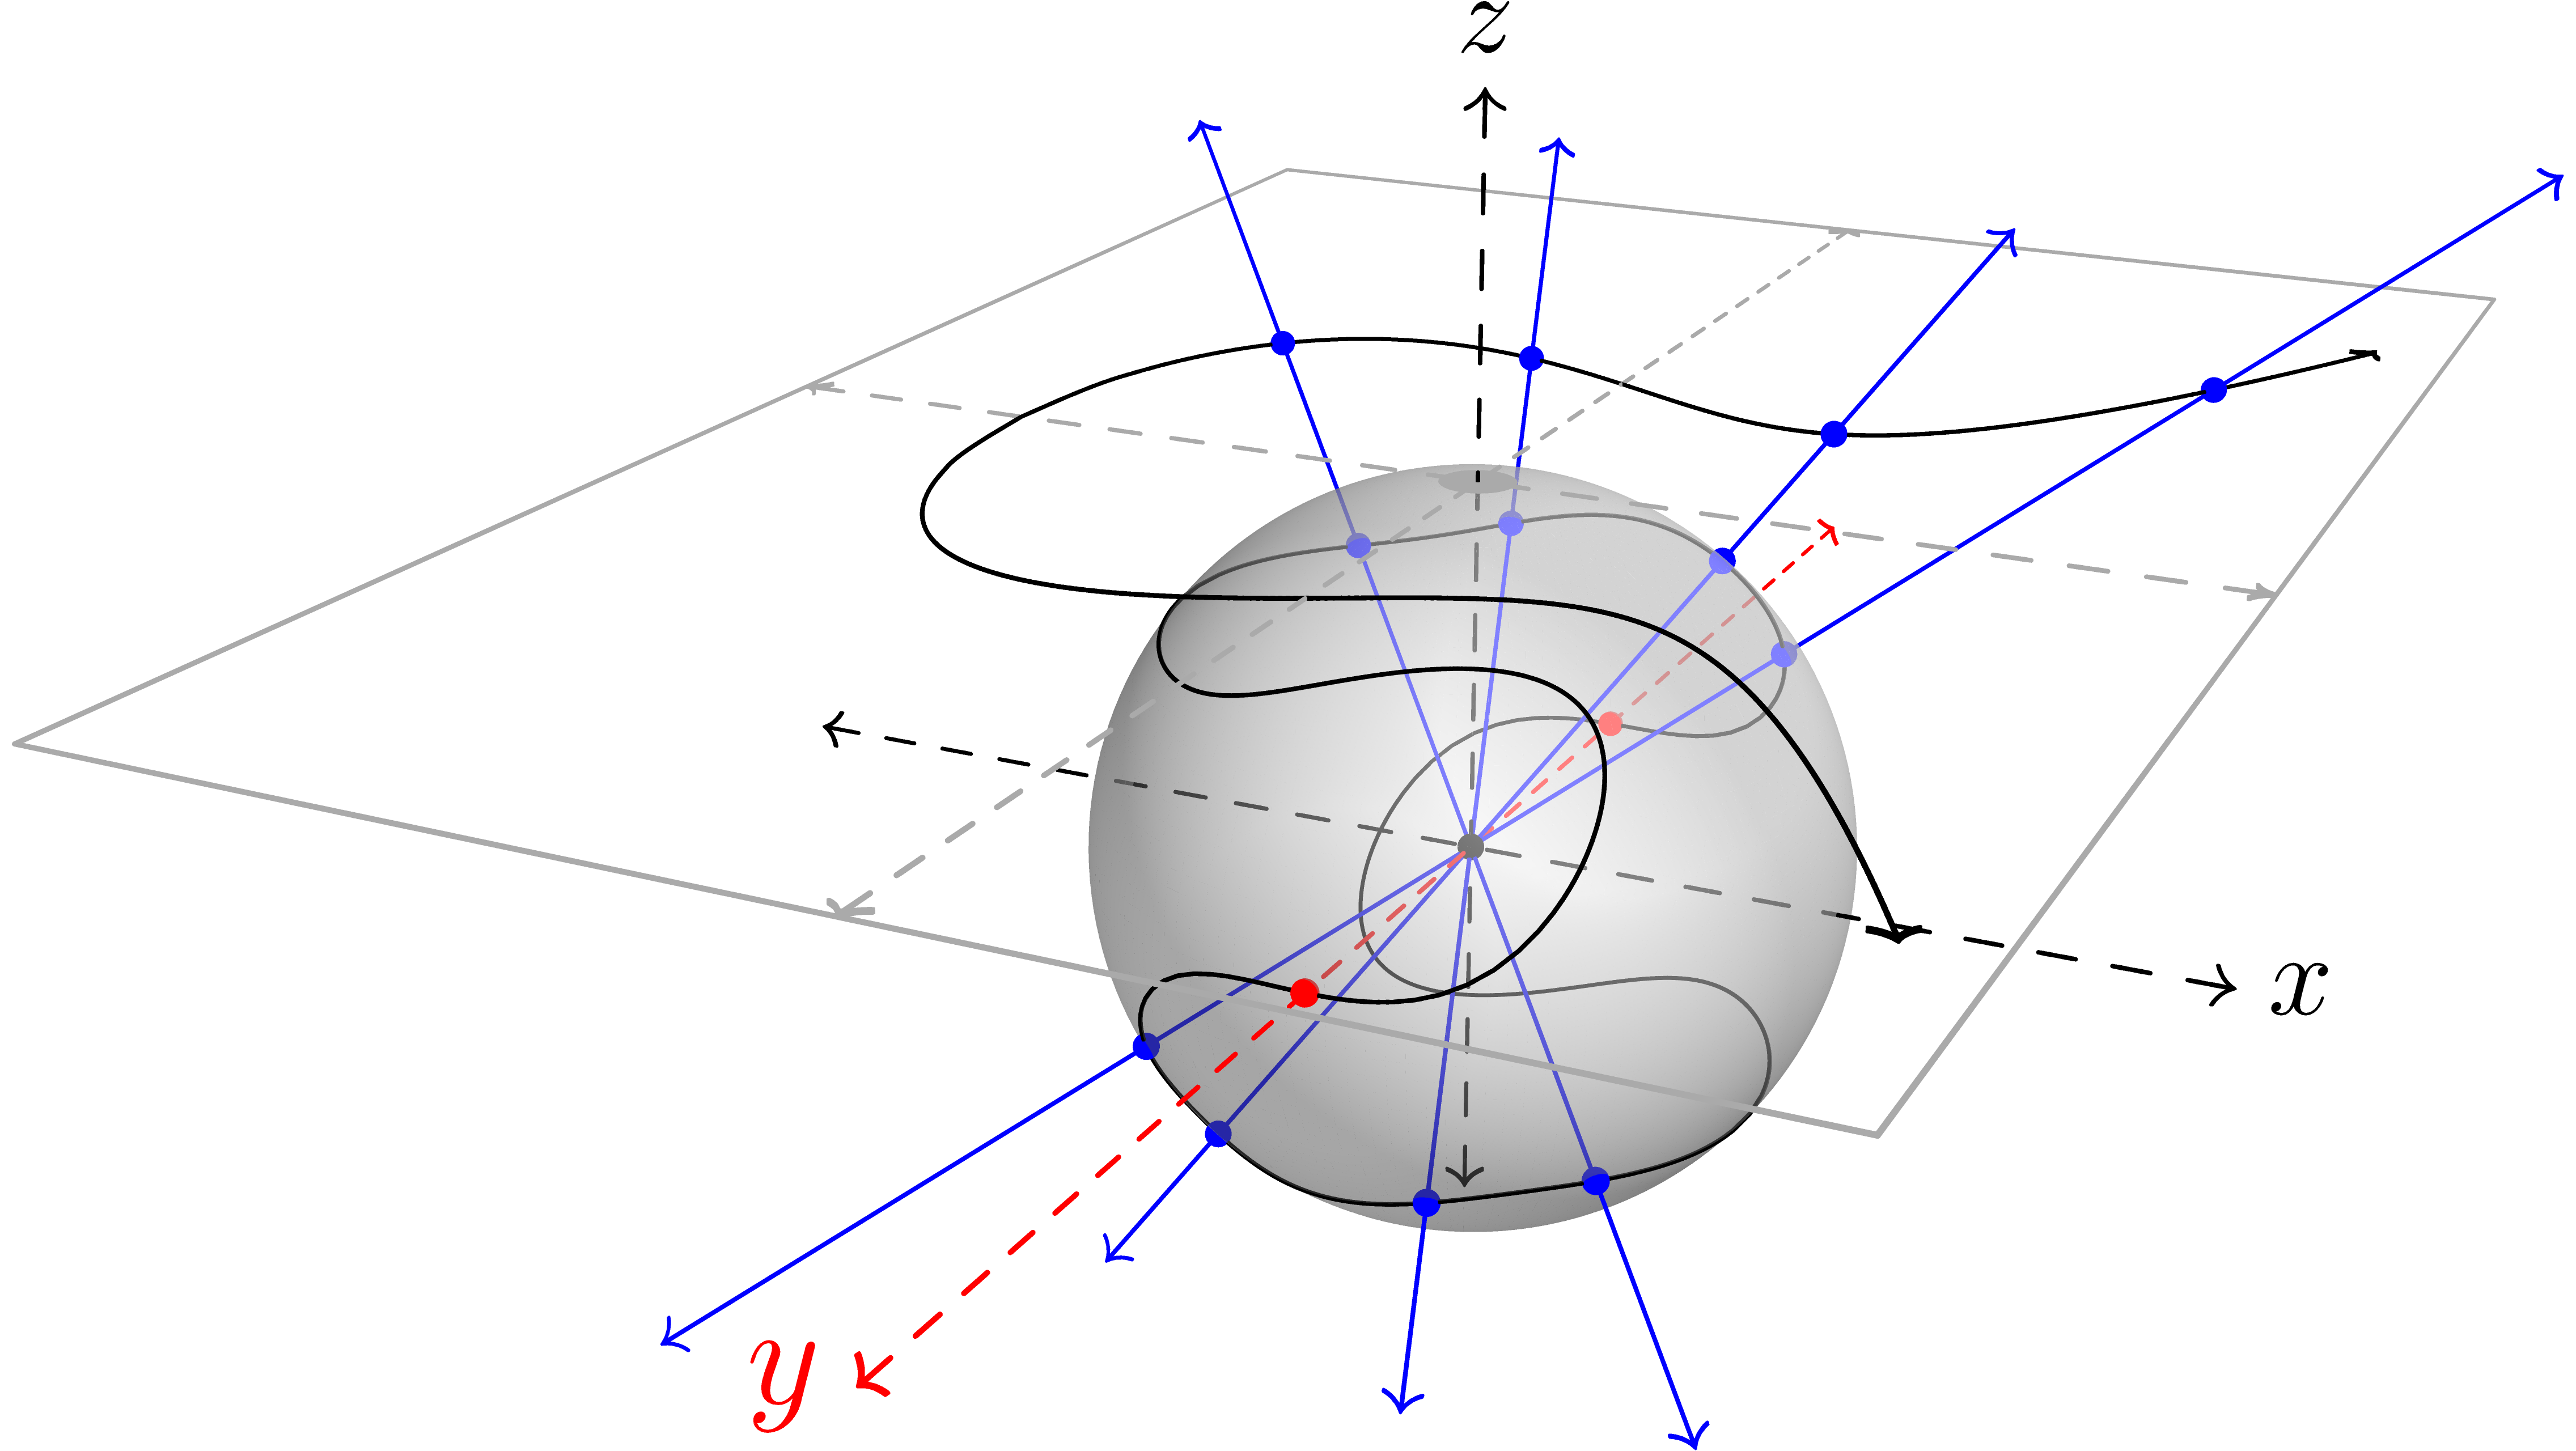
\includegraphics[width=0.8\textwidth]{projectivePlanInfinityPoint}
            \caption{Elliptic curve of equation $y^2 = x^3 -x +1$ on the projective plane}
            \label{fig:courbePlanProjectif}
        \end{figure}
\end{frame}
